% vim:nojs:spelllang=en_au tw=76 sw=4 sts=4 fo+=awn fmr={-{,}-} et ts=8
\documentclass[11pt,a4paper]{article}
\usepackage{isabelle,isabellesym}

\usepackage{amssymb}
\usepackage[only,bigsqcap]{stmaryrd}

\usepackage{mathpartir}
\usepackage[margin=10mm,bottom=15mm]{geometry}
\usepackage[final]{graphicx}

% this should be the last package used
\usepackage{pdfsetup}

% urls in roman style, theory text in math-similar italics
\urlstyle{rm}
\isabellestyle{rm}

\begin{document}

\title{Mechanization of the Algebra for Wireless Networks (AWN)}
\author{Timothy Bourke\thanks{Inria, \'Ecole normale sup\'erieure, and 
NICTA}}
\maketitle

\begin{abstract}
AWN is a process algebra developed for modelling and analysing protocols for 
Mobile Ad hoc Networks (MANETs) and Wireless Mesh Networks 
(WMNs)~\cite[\textsection 4]{FehnkerEtAl:AWN:2013}.
AWN models comprise five distinct layers: sequential processes, local 
parallel compositions, nodes, partial networks, and complete networks.

This development mechanises the original operational semantics of AWN and 
introduces a variant `open' operational semantics that enables the 
compositional statement and proof of invariants across distinct network 
nodes.
It supports labels (for weakening invariants) and (abstract) data state 
manipulations.
A framework for compositional invariant proofs is developed, including a 
tactic (\verb|inv_cterms|) for inductive invariant proofs of sequential 
processes, lifting rules for the open versions of the higher layers, and a 
rule for transferring lifted properties back to the standard semantics.
A notion of `control terms' reduces proof obligations to the subset of 
subterms that act directly (in contrast to operators for combining terms and 
joining processes).

Further documentation is available in~\cite{BourkeEtAl:MechAWN:2014}.

\centering{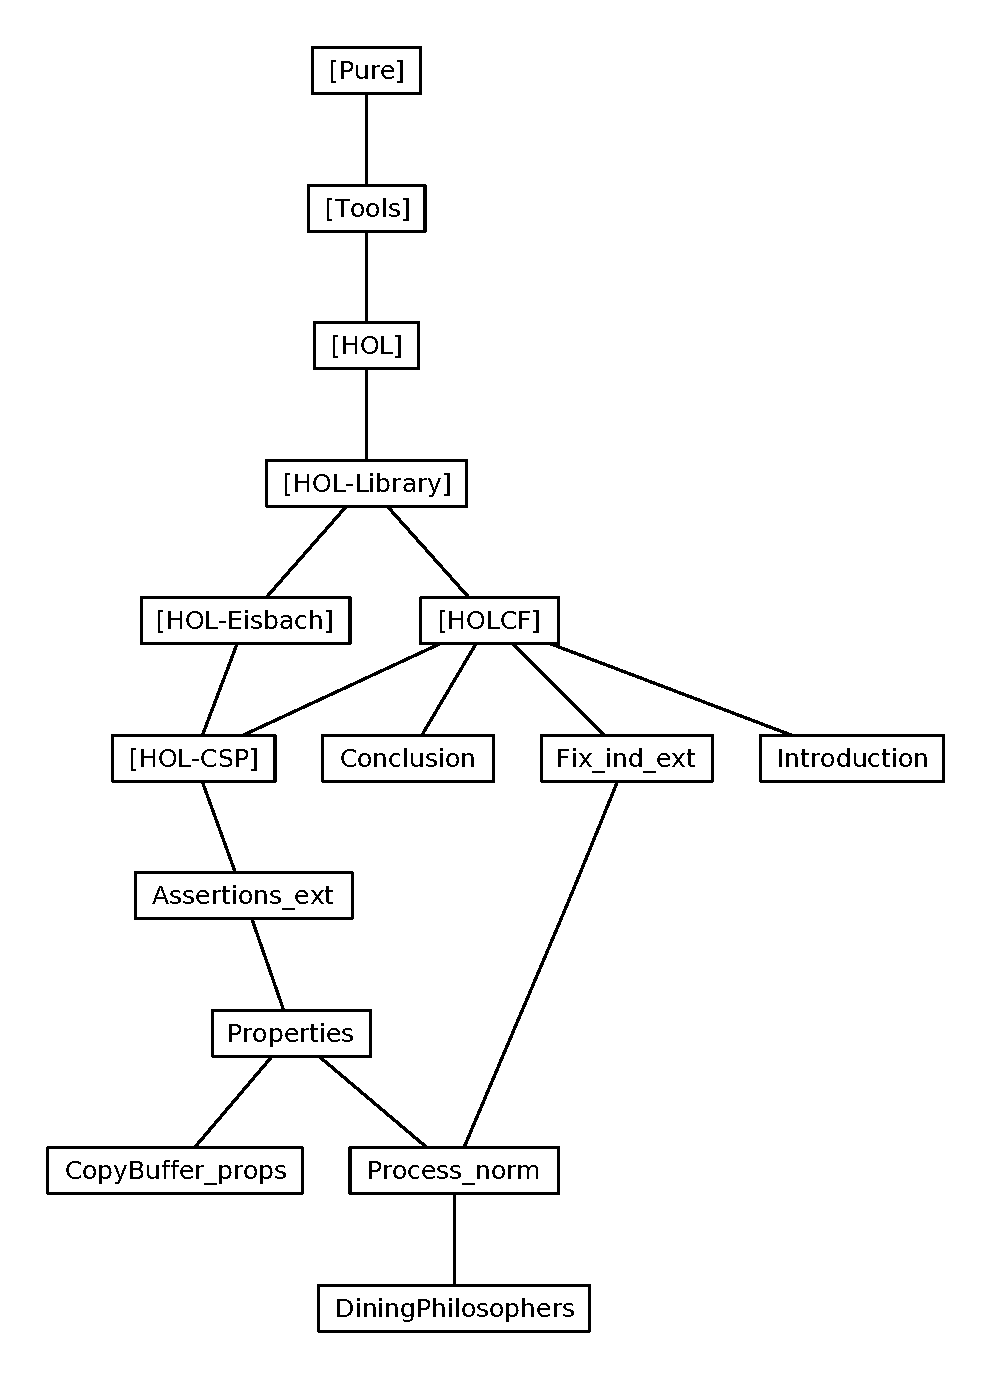
\includegraphics[width=.6\textwidth]{session_graph}}
\end{abstract}

\tableofcontents

% sane default for proof documents
\parindent 0pt\parskip 0.5ex

% generated text of all theories
\newpage
\input{session}

\section{Acknowledgements}

We thank Peter H\"ofner for agreeing to the inclusion of the simple `Toy' 
example model.

% optional bibliography
\bibliographystyle{abbrv}
\bibliography{root}

\end{document}
